\renewcommand{\luku}[2]{\section{#2} \lukufilter{#1}{\input{maa2/TEORIA_#1} \input{maa2/TEHT_#1}}} % luku
\renewcommand{\nluku}[2]{\section*{#2} \addcontentsline{toc}{section}{#2} \lukufilter{#1}{\input{maa2/#1}}} % numeroimaton luku

\newpage
\nosa{MAA2 -- Polynomifunktiot}
\lukufilter{#1}{Polynomit ovat hyvin keskeisiä sovelletussa matematiikassa. Niin fysiikan, kemian, tietotekniikan kuin myös taloustieteiden parissa varsin monet laskutoimitukset pelkistyvät lopulta polynomien käsittelyksi. Esimerkiksi sellaiset tietotekniset sovellutukset kuten hahmon tunnistaminen kuvasta, äänen kompressointi (mp3) ja vaikkapa sikiön sydänäänien erottaminen perustuvat lopulta polynomien laskentaan. Itse asiassa polynomit ovat niin yleisiä matematiikassa, että riippumatta sovellusalueesta ne on hyvä tuntea perusteellisesti.

Pitkän matematiikan toisella kurssilla MAA2 Polynomifunktiot käsitellään polynomifunktioita, -yhtälöitä ja -epäyhtälöitä. Kurssilla syvennetään ensimmäisen kurssin asioita ja sovelletaan niitä polynomien maailmassa. Oppikirja on rakennettu siten, että aiheet esitellään lukujen alussa ja havainnollistetaan esimerkein. Tehtäviä on runsaasti ja niiden tarkoituksena on saada opiskelija sisäistämään opiskellut asiat ja siirtämään ne käytäntöön.

Tässä kirjassa käymme läpi opetussuunnitelman mukaiset keskeiset sisällöt, joita ovat
\luettelo{
§ polynomien tulo ja binomikaavat
§ polynomifunktio
§ toisen ja korkeamman asteen polynomiyhtälöt
§ toisen asteen yhtälön juurten lukumäärän tutkiminen
§ polynomiepäyhtälön ratkaiseminen
}

Opetussuunnitelman mukaiset kurssin keskeiset tavoitteet ovat, että opiskelija
\luettelo{
§ harjaantuu käsittelemään polynomifunktioita
§ oppii ratkaisemaan toisen asteen polynomiyhtälöitä ja tutkimaan ratkaisujen lukumäärää
§ oppii ratkaisemaan korkeamman asteen polynomiyhtälöitä, jotka voidaan ratkaista ilman polynomien jakolaskua
§ oppii ratkaisemaan yksinkertaisia polynomiepäyhtälöitä
}

%tähtitehtävät -> valaistuminen}

\osa{Polynomi}
    \luku{polynomi}{Polynomi}
    \luku{polynomien_kertolasku}{Polynomeilla laskeminen}
    \luku{muistikaavat}{Muistikaavat}
    \luku{tulon_nollasaanto_ja_tulon_merkkisaanto}{Tulon nollasääntö \& tulon merkkisääntö}
    \luku{tekijoihinjako}{Polynomin jakaminen tekijöihin}
    \luku{polynomifunktion_kuvaaja}{Polynomifunktion kuvaaja}

\osa{Ensimmäinen aste}
    \luku{epayhtalo}{Epäyhtälöiden teoriaa}
    \luku{ensimmaisen_asteen_yhtalo}{Kertausta: ensimmäisen asteen yhtälö}
    \luku{ensimmaisen_asteen_epayhtalo}{Ensimmäisen asteen epäyhtälö}

\osa{Toinen aste}
    \luku{paraabeli}{Toisen asteen polynomifunktio ja sen kuvaaja}
    \luku{toisen_asteen_yhtalo}{Toisen asteen yhtälö}
    \luku{toisen_asteen_yhtalon_ratkaisukaava}{Toisen asteen yhtälön ratkaisukaava}
    \luku{diskriminantti}{Diskriminantti}
    \luku{toisen_asteen_epayhtalo}{Toisen asteen epäyhtälö}
    \luku{jakolause}{Polynomien jakolause}
    
\osa{Korkeampi aste}
    \luku{korkeamman_asteen_polynomifunktio}{Korkeamman asteen polynomifunktio}
    \luku{korkeamman_asteen_yhtalot}{Korkeamman asteen yhtälöt}
    \luku{korkeamman_asteen_epayhtalot}{Korkeamman asteen epäyhtälöt}

\newpage
\osa{Kertausosio}
   \nluku{LIITE_testaatietosi}{Testaa tietosi!}
   \nluku{LIITE_kertausteht}{Kertaustehtäviä}
   \newpage
   \nluku{LIITE_harjoituskokeita}{Harjoituskokeita}
   \nluku{LIITE_yokokeita}{Ylioppilaskoetehtäviä}

\chapter*{Syventäviä aiheita}
\addcontentsline{toc}{chapter}{Syventäviä aiheita}
    \section*{Lukujärjestelmät} \addcontentsline{toc}{section}{Lukujärjestelmät} \lukufilter{LIITE_lukujarjestelmat}{\subsection*{Paikkajärjestelmät}

Merkitsemme lukuja yleensä \termi{kymmenjärjestelmä}{kymmenjärjestelmässä} eli \termi{lukujärjestelmä}{lukujärjestelmässä}, jossa on kymmenen \termi{numeromerkki}{numeromerkkiä}: 0, 1, 2, 3, 4, 5, 6, 7, 8 ja 9. (Käyttämämme numeromerkit ovat nimeltään hindu-arabialaiset numerot.) Kymmenjärjestelmää kutsutaan myös \termi{desimaalijärjestelmä}{desimaalijärjestelmäksi}. Tunnetaan kulttuureja, joissa on käytetty pääasiallisesti jotakin muuta lukujärjestelmää.

Kymmenjärjestelmä on \termi{paikkajärjestelmä}{paikkajärjestelmä}, eli merkin paikka määrittää sen merkityksen.

\begin{esimerkki}
Numeron 8 merkitys riippuu sen paikasta. Luvussa $80$ merkin 8 merkitys on $8 \cdot 10^1$, mutta luvussa $820$ sen merkitys on $8 \cdot 10^2$.
\end{esimerkki}
%viittaus desimaalilukukappaleeseen?
\begin{esimerkki}
Esitä luku $2\,080,7$ kymmenen potenssien summana.
	\begin{esimratk}
	$2\,090,7=2\cdot10^3+0\cdot10^2+0\cdot10^1+0\cdot10^0+7\cdot10^{-1}$
	\end{esimratk}
\end{esimerkki}

Nykyään yleisimmät desimaalijärjestelmästä poikkeavat lukujärjestelmät ovat \termi{binäärijärjestelmä}{binääri}-, \termi{oktaalijärjestelmä}{oktaali}- ja \termi{heksadesimaalijärjestelmä}{heksadesimaalijärjestelmät}, joissa on vastaavasti $2$, $8$ ja $16$ numeromerkkiä. Tietokoneet käsittelevät lukuja sisäisesti binäärijärjestelmässä, kun taas oktaali- ja heksadesimaalijärjestelmät ovat muutoin käteviä tietojenkäsittelytieteessä.

Yleisesti pätee, että kun käytettävissä olevien merkkien määrää lisää, suuria lukuja voi kirjoittaa lyhyempään muotoon. Näin ollen sama luku esitettynä kolmekantaisessa lukujärejstelmässä voi olla paljon pidempi kuin kymmenkantaisessa esitettynä. Tilanne on verrattavissa vaikkapa kiinan kieleen, jossa on käytössä tuhansia erilaisia kirjoitusmerkkejä. Merkeissä on paljon muistettavaa, mutta toisaalta kokonaisen lauseen voi kirjoittaa vain parilla kirjoitusmerkillä.

Binäärijärjestelmässä luvun muodostavia numeromerkkejä kutsutaan \termi{bitti}{biteiksi}. Bitti voi olla joko päällä (1) tai pois päältä (0), ja toteutus tietokoneessa vastaa esimerkiksi sitä, että johtimessa kulkee virta (1) tai ei (0). Kuusitoistajärjestelmässä tarvitaan numeroiden $0 \ldots \, 9$ lisäksi kuusi uutta numeromerkkiä. Tavaksi on vakiintunut käyttää kirjainmerkkejä $\mathrm{A, B, C, D, E, F}$. Ne vastaavat desimaalilukuja $10 \ldots \, 15$.

Useampaa järjestelmää käytettäessä, erityisesti muunnettaessa lukuja järjestelmästä toiseen, merkitään kantaluku luvun jälkeen alaindeksinä. Voimme esimerkiksi merkitä (desimaalijärjestelmän) lukua yhdeksäntoista $10011_2$, $23_8$, $19_{10}$ tai $13_{16}$. Huomaa, että binäärijärjestelmän luvuissa ei ole mielekästä käyttää tuhaterotinta, koska sana tuhat itsessään viittaa kymmenjärjestelmälle ominaiseen kolmanteen kymmenen potenssiin. Binääriluvuille ei ole vakiintunut vastaavia ilmaisuja kuten sata tai miljoona, vaan luvut luetaan numero kerrallaan.

\begin{esimerkki}
Luku $11001_2$ luetaan "yksi yksi nolla nolla yksi".
\end{esimerkki}

Luvut eri kannoissa voidaan muuttaa desimaaliluvuiksi esittämällä luku potenssien summina kymmenjärejstelmässä.

%alaviitemerkintä

\begin{esimerkki}
$10,01_2 = 1 \cdot 2^1 + 0 \cdot 2^0 + 0 \cdot 2^{-1} + 1 \cdot 2^{-2} = 2,25_{10}$
\end{esimerkki} %pitää kirjoittaa näitä muunnosesimerkkejä :/

%\begin{esimerkki}
%Millä kantaluvulla $n$ pätee yhtälö $10_n+10_n=$ ... (tulee potensisyhtälö,tuntematon kantaluku)
%\end{esimerkki}

Lukujärjestelmiä voidaan vaihtoehtoisesti merkitä kirjoittamalla niiden tunnus (Bin, Oct, Dec, Hex) luvun jälkeen. Klassinen vitsi ''Miksi tietojenkäsittelytieteilijä sekoittaa halloweenin ja joulun? Koska $31$ Oct $= 25$ Dec!'' perustuu siihen, että

\begin{align*}
	\text{halloween} \; = \; \text{31. lokakuuta} \; &= \; \text{31 Oct} \; = 31_8 = 3_{10} \cdot 8_{10} + 1_{10} \cdot 1_{10} \\
	= {25}_{10} &= \; \text{25 Dec} \; = \; \text{25. joulukuuta} \; = \; \text{joulupäivä.}
\end{align*} %välit, siistimistä?

\subsection*{Muut lukujärjestelmät}

Yleisesti tunnetaan myös joitakin lukujärjestelmiä, jotka eivät ole paikkajärjestelmiä.

\termi{tukkimiehen kirjanpito}{Tukkimiehen kirjanpidossa} toistetaan yhtä ainoaa merkkiä. Se on tavallaan 1-järjestelmä, mutta tällainen määrittely ei ole ongelmaton.

\begin{center}
	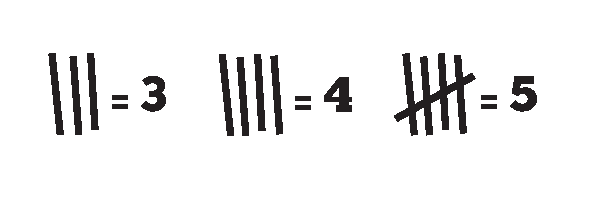
\includegraphics{pictures/Kuva1-1-tukkimiehenkirjanpito.pdf}
\end{center}

Hienostuneempi versio tukkimiehen kirjanpidosta ovat \termi{roomalaiset luvut}{roomalaiset luvut}, jotka nimensä mukaisesti olivat yleisin lukujärjestelmä antiikin Roomassa. Roomalaisia lukuja käytetään yhä nykyäänkin erityisesti järjestyksen merkitsemisessä. Roomalaisten lukujen numeromerkit ovat I, V, X, L, C, D ja M. Ne vastaavat desimaalijärjestelmän lukuja seuraavalla tavalla:

\begin{equation*}
	\textrm{I}=1\quad
	\textrm{V}=5\quad
	\textrm{X}=10\quad
	\textrm{L}=50\quad
	\textrm{C}=100\quad
	\textrm{D}=500\quad
	\textrm{M}=1\,000
\end{equation*}

Roomalaiset luvut merkitään kirjoittamalla merkkejä laskevassa järjestyksessä, poikkeuksena vähennyssääntö. Merkkien kokonaisarvo määrää luvun. Vähennyssääntö tarkoittaa kuutta kaksimerkkistä ilmaisua:

\begin{equation*}
	\textrm{IV}=4\quad
	\textrm{IX}=9\quad
	\textrm{XL}=40\quad
	\textrm{XC}=90\quad
	\textrm{CD}=400\quad
	\textrm{CM}=900
\end{equation*}

Joissain vanhoissa teksteissä (ja jopa kellotauluissa) luku $4$ on merkitty myös IIII.

Luvussa voi olla vain kerran IV tai IX, vain kerran XL tai XC ja vain kerran CD tai CM. Kaksimerkkisiin ilmaisuihin pätevät samat säännöt kuin numeromerkkeihinkin: I$=1$ ei voi edeltää numeroa IV$=4$, eikä IV$=4$ numeroa V$=5$. Lisäksi merkinnät IXV, XCL ja CMD eivät ole sallittuja. Oikea roomalainen luku minimoi käytettyjen merkkien määrän. Esimerkiksi VIV ei ole roomalainen luku, sillä IX on esityksenä lyhyempi.

\termi{nolla}{Nollaa} roomalaisissa numeroissa ei ole; nolla nykyisessä merkityksessään kehitettiin vasta Intiassa 800-luvulla jaa.

\newpage % VIIMEISTELY
\begin{esimerkki}
	Roomalaisia lukuja:
	\alakohdat{
		§ III$=1+1+1=3$
		§ IX$=10-1=9$
		§ XII$=10+1+1=12$
		§ XIV$= 10 + (5 - 1) = 14$
		§ CDX$=500-100+10=410$
		§ MDC$=1\,000+500+100=1\,600$
	}
\end{esimerkki}

\begin{tehtavasivu}

\begin{tehtava}
Muunna seuraavat binääriluvut kymmenjärjestelmään.
	\alakohdat{
		§ $101,0_2$
		§ $1,00101_2$
		§ $100101,1101_2$
	}
\begin{vastaus}
	\alakohdatm{
		§ $5,0_{10}$
		§ $1,15625_{10}$
		§ $37,8125_{10}$
	}
\end{vastaus}
\end{tehtava}

\begin{tehtava}
Muunna seuraavat luvut binäärijärjestelmään.
	\alakohdatm{
		§ $7,0_{10}$
		§ $2,5_{10}$
		§ $11,1875_{10}$
	}
\begin{vastaus}
	\alakohdatm{
		§ $111,0_2$
		§ $10,1_2$
		§ $1011,0011_2$
	}
\end{vastaus}
\end{tehtava}

\begin{tehtava}
Muuta seuraavat kymmenjärjestelmän luvut heksadesimaaliluvuiksi.
\alakohdat{§ $175$ § $384$}
\end{tehtava}

\begin{tehtava}
	Laske
	\alakohdat{
		§ $1101_2 \cdot 100_2$ %joskus tulevaisuudessa meillä on esimerkkejä jakokulmasta binääriluvuille ;_;
		§ $1101001_2 \cdot 100000_2$
		§ $10110_2 \cdot 0,01_2$.
	}
	\begin{vastaus}
		\alakohdat{
			§ $110100_2$
			§ $110100100000_2$
			§ $101,1_2$
		}
	\end{vastaus}
\end{tehtava}

\begin{tehtava}
Mitkä seuraavista ovat oikeita roomalaisia lukuja? Mitä ne ovat kymmenjärjestelmässä?
\alakohdatm{
§ CLI
§ IVX
§ VIZI
§ CCLI
§ CCCLXXXVI
§ CMVCI
§ MMDCXLIIII
§ CDXCIII
§ DCXLIX
} 
\begin{vastaus}
\alakohdatm{
§ $151$
§ Ei ole oikea roomalainen luku.
§ Ei ole oikea roomalainen luku.
§ $251$
§ $386$
§ Ei ole oikea roomalainen luku.
§ Ei ole oikea roomalainen luku.
§ $493$
§ $649$
}
\end{vastaus}
\end{tehtava}

\begin{tehtava}
Muuta seuraavat kymmenjärjestelmän luvut roomalaisiksi luvuiksi. Kuinka monta merkkiä tarvitaan luvun kirjoittamiseen?
\alakohdatm{
§ $278$
§ $712$
§ $1\,478$
§ $3\,999$
}
\begin{vastaus}
\alakohdat{
§ CCLXXVIII, $9$ merkkiä 
§ DCCXII, $6$ merkkiä
§ MCDLXXVIII, $10$ merkkiä
§ MMMCMXCIX, $9$ merkkiä
}
\end{vastaus}
\end{tehtava}

\begin{tehtava}
Tunnetusti $10\cdot 10=100$. Samannäköiseen tuloon päädytään myös, vaikka luku tulkittaisiin kaksikantaisena: $10_2 \cdot 10_2 = 2_{10}\cdot 2_{10}=4_{10}=100_2$. Tutki, päteekö tulo yleisesti, eli onko $10_n\cdot 10_n = 100_n$ myös kaikilla $n >2$.
	\begin{vastaus}
$10_n=1\cdot n^1+0\cdot n^0=n$, eli $10_n \cdot 10_n =n\cdot n = n^2= 1\cdot n^2 + 0 \cdot n^1 + 0\cdot n^0 =100_n$. Väite siis pätee kaikilla kantaluvuilla. (Huomaa, että välivaiheiden eksponentit ja kertoimet ovat kymmenjärjestelmän lukuja.)
	\end{vastaus}
\end{tehtava}

\begin{tehtava}
Muodosta kertotaulu binääriluvuille $1$--$100$.
	\begin{vastaus}
\begin{tabular}{|c||c|c|c|c|}
	\hline 
	$\cdot$ & $1$ & $10$ & $11$ & $100$ \\
	\hline
	\hline
	$1$ & $1$ & $10$ & $11$ & $100$ \\
	\hline 
	$10$ & $10$ & $100$ & $110$ & $1000$  \\
	\hline 
	$11$ & $11$ & $110$ & $1001$ & $1010$ \\
	\hline 
	$100$ & $100$ & $1000$ & $1010$ & $10000$ \\
	\hline 
	\end{tabular} 	
	\end{vastaus}
\end{tehtava}

\begin{tehtava}
	$\star$ Mikä on suuruusjärjestyksessä $148$. positiivinen kokonaisluku, jonka kymmenjärjestelmäesityksessä on vain nollia ja ykkösiä?
	\begin{vastaus}
		$10\,010\,100$
	\end{vastaus}
\end{tehtava}

%\begin{tehtava}
%tallennustilasta, kuinka paljon tilaa tarvitaan tallentaamaan jokin luku halutullal tarkkuudella binäärijärejstelmäääs
%	\begin{vastaus}
%
%	\end{vastaus}
%\end{tehtava}

\end{tehtavasivu}}
    \section*{Paraabeli} \addcontentsline{toc}{section}{Paraabeli} \lukufilter{LIITE_paraabeli}{\subsection*{Toisen asteen polynomin kuvaaja}
\label{paraabeli_tod}

Tässä liitteessä perustellaan, miksi kaikkien toisen asteen polynomifunktioiden kuvaajat näyttävät samalta. Lisäksi tarkastellaan, mitkä tekijät vaikuttavat kuvaajien muotoon.

\underline{Funktio $P(x)=x^2$}

Aloitetaan funktiosta $P(x)=x^2$. Mitä tiedämme siitä piirtämättä kuvaajaa?
\luettelo{
§ Algebrallisen päättelyn avulla voimme todeta, että funktion pienin arvo on $P(0) = 0$, sillä tulon merkkisäännön perusteella lauseke $x^2$ ei voi saada negatiivisia arvoja – ei ole olemassa sellaista reaalilukua $x$, jonka neliö olisi negatiivinen. (Kompleksiluvuilla tällaista rajoitusta ei ole, tästä lisää liitteessä.) Kuvaajan alin kohta sijoittuu siis origoon ja kuvaajan kaikki muut pisteet sen yläpuolelle.
§ Kun $x > 0$, lauseke $x^2$  on sitä
suurempi, mitä suurempi $x$ on. Tästä tiedämme, että nollasta oikealle siirryttäessä funktion kuvaaja nousee.
§ Koska $(-x)^2 = x^2$, kuvaaja on symmetrinen $y$-akselin suhteen.
}

Näiden tietojen avulla voimme päätellä, että funktion kuvaaja koostuu kahdesta
identtisestä haarasta, jotka kohtaavat, kun $x=0$. Mitä kauempana $x$ on nollasta, sitä suurempia ovat funktion arvot. Tämän kaiken voi päätellä jo ennen kuvaajan piirtämistä.

Merkitsemällä koordinaatistoon yhtälön $y=x^2$ toteuttavia pisteitä, muodostuu lopulta funktion kuvaaja:
\begin{center}
\begin{kuvaajapohja}{2}{-2}{2}{-1}{4}
  \kuvaaja{x**2}{$f(x)=x^2$}{blue}
\end{kuvaajapohja}
\end{center}

% FIXME: ongelmallista: ''alaspäin aukeava'' vasta seuraavaksi
Kuvaajan muoto on geometriselta nimeltään \emph{paraabeli}. Paraabeleja esiintyy monessa yhteydessä: esimerksi polttopeilin ja radioteleskoopin pinta kaareutuu paraabelin muotoisena. Samoin ilmaan heitetyn kappaleen rata on likimain alaspäin aukeava paraabeli, kun ilmanvastus on pieni.

\underline{Funktio $P(x)=ax^2, \quad a\neq 0$}

Polynomien $P(x)=ax^2$ arvot ovat ovat lausekkeeseen $x^2$ nähden $a$-kertaisia. Muuten paraabelin symmetrisyys ja muut keskeiset ominaisuudet säilyvät.

\luettelo{
§ Kun $a > 0$, myös $ax^2\geq 0$, joten pienin arvo on yhä $0$.\\
Paraabeli on \termi{ylöspäin aukeava}{ylöspäin aukeava}.
§ Kun $a < 0$, tulon merkkisäännön nojalla $ax^2 \leq 0$. \\
 Nyt $P(0)=0$ onkin suurin arvo, ja funktion arvot ovat sitä pienempiä,
mitä enemmän $x$ poikkeaa nollasta. \\
Paraabeli on \termi{alaspäin aukeava}{alaspäin aukeava}.
§ Mitä enemmän $a$ poikkeaa nollasta, sitä nopeammin funktion arvot
muuttuvat $x$:n muuttuessa ja sitä kapeampi paraabeli on.
}

\begin{center}
$a>0$, paraabeli aukeaa ylöspäin:\\
\begin{tabular}{cc}
$f(x)=\frac{1}{2}x^2$& $f(x)=2x^2$ \\
\begin{kuvaajapohja}{1}{-2}{2}{-1}{4}
  \kuvaaja{0.5*x**2}{}{blue}
\end{kuvaajapohja} &
\begin{kuvaajapohja}{1}{-2}{2}{-1}{4}
  \kuvaaja{2*x**2}{}{blue}
\end{kuvaajapohja}
\end{tabular}

$a<0$, paraabeli aukeaa alaspäin:\\
\begin{tabular}{cc}
$f(x)=-\frac{1}{2}x^2$ & $f(x)=-2x^2$ \\
\begin{kuvaajapohja}{1}{-2}{2}{-4}{1}
  \kuvaaja{-0.5*x**2}{}{blue}
\end{kuvaajapohja} &
\begin{kuvaajapohja}{1}{-2}{2}{-4}{1}
  \kuvaaja{-2*x**2}{}{blue}
\end{kuvaajapohja}
\end{tabular}
\end{center}

\underline{Funktio $P(x)=ax^2+c$}

Lisäämällä vakiotermi $c$ saadaan $P(x)=ax^2+c$. Vakion lisääminen nostaa tai laskee funktion kuvaajaa (riippuen siitä, onko $c > 0$ tai $c<0$), joten kuvaajan muoto ei muutu.

\underline{Funktio $P(x)=ax^2+bx+c$}

Miksi sitten täydellisen toisen asteen polynomin $P(x)=ax^2+bx+c$ kuvaaja on myös paraabeli? Muokataan lauseketta, aloitetaan ottamalla yhteinen tekijä:
\begin{align*}
P(x) &=ax^2+bx+c \\
&= a\left(x^2 +\frac{b}{a}x\right) + c  \quad &
\text{ lavennetaan } \frac{b}{a} \text{ kahdella} \\
&= a\left(x^2 +2\cdot x \cdot \frac{b}{2a} \quad\right) + c  &
\text{ täydennetään neliöksi lisäämällä} \left( \frac{b}{2a} \right)^2 \\
&= a \Bigg( \underbrace{x^2 +2\cdot x \cdot \frac{b}{2a}+\left(\frac{b}{2a} \right)^2}_{\left( x+\frac{b}{2a} \right)^2}
- \left(\frac{b}{2a}\right)^2 \Bigg)  + c \\
&= a \left( \left( x + \frac{b}{2a} \right )^2-\frac{b^2}{4a^2} \right) + c &
\text{ kerrotaan sulut auki } \\
&= a \underbrace{\left(  x + \frac{b}{2a} \right)^2}_{\text{neliö}}-
\underbrace{\frac{b^2}{4a} + c}_{\text{vakio}}
\end{align*}

Tästä neliöksi täydennetyksi muodosta nähdään, että $P(x)$ on muotoa
$a\cdot$neliö + vakio. Kuvaaja on siis samanlainen kuin tapauksessa
$ax^2+c$, huippu on vain siirtynyt.
Koska neliö $\geq 0$, saadaan

\luettelo{
§ Kun $a>0$, kyseinen vakio on polynomin pienin arvo ja kuvaaja on
ylöspäin aukeava paraabeli.
§ Kun $a<0$, kyseinen vakio on suurin arvo ja kuvaaja on alaspäin
aukeava paraabeli.
}

Paraabelin \termi{huippu}{huippu} (eli kuvaajan piste, jossa suurin tai pienin arvo
saavutetaan) on aina kohdassa
$x=-\frac{b}{2a}$, koska silloin neliö on nolla.

%Toisen asteen polynomifunktio on muotoa $f(x)=ax^2+bx+c$, jossa $a,b,c \in \R$ ja $a \neq 0$. Toisen asteen polynomifunktion kuvaaja on paraabeli. Toisen asteen polynomifunktioita käytetään matemaattisessa mallinnuksessa talouden, tieteen ja tekniikan aloilla. Esimerkiksi heittoliikkeessä olevan kappaleen lentorata on aina paraabelin muotoinen. \\
%\textbf{Esimerkki 1.}
%a) Piirrä funktion $f(x)=x^2-2$ kuvaaja. \\
%b) Ratkaise funktion $f$ nollakohdat. \\ \\
%
%\begin{kuvaajapohja}{1}{-2}{2}{-3}{1}
%  \kuvaaja{x**2-2}{$f(x)=x^2-2$}{blue}
%\end{kuvaajapohja}
%
%Funtkion kuvaaja on ylöspäin aukeava paraabeli, joka leikkaa x-akselin kohdissa joissa $f(x)=0$. \\
%Graafisesti funktion nollakohdat saadaan ratkaistua kuvaajasta. Kuvaajasta nähdään, että funktion nollakohdat ovat $x_1 \approx 1,4$ ja $x_2 \approx -1,4$. \\
%Algebrallisesti saadaan ratkaistua, että funktion nollakohdat ovat
%\begin{align*}
%f(x)&=0 \\
%x^2-2&=0 \\
%x^2&=2 \\
%x&= \pm \sqrt[]{2}
%\end{align*}
%Funktion $f$ kuvaajasta huomataan, että se on symmetrinen y-akselin suhteen.
%
%\textbf{Esimerkki 2.} \\
%Piirrä funktioiden $f(x)=x^2+1$, $g(x)=2x^2$ ja $h(x)=\frac{1}{3}x^2$ kuvaajat. \\ \\
%
%\begin{kuvaajapohja}{1}{-2}{2}{-1}{3}
%  \kuvaaja{x**2+1}{$f(x)=x^2+1$}{blue}
%\end{kuvaajapohja}
%
%
%\begin{kuvaajapohja}{1}{-2}{2}{-1}{3}
%  \kuvaaja{2*x**2}{$g(x)=2x^2$}{blue}
%\end{kuvaajapohja}
%
%\begin{kuvaajapohja}{1}{-2}{2}{-1}{3}
%  \kuvaaja{(1 / 3.0)*(x**2)}{$h(x)=\frac{1}{3}x^2$}{blue}
%\end{kuvaajapohja}
%
%Mitä tapahtuu funktion kuvaajan muodolle, kun termin $ax^2$ kerroin $a$ muuttuu? \\ \\
%
%\textbf{Esimerkki 3.} \\
%Piirrä funktioiden $f(x)=-x^2+x$, $g(x)=-x^2+2x+1$ ja $h(x)=-x^2+\frac{1}{2}x-1$ kuvaajat. \\
%\missingfigure \\
%Mitä tapahtuu funktion kuvaajan muodolle, kun termin $bx$ kerroin $b$ muuttuu? \\ \\
%
%\textbf{Esimerkki 4.} \\
%Piirrä funktioiden $f(x)=x^2$, $g(x)=x^2-2$ ja $h(x)=x^2+\frac{3}{2}$ kuvaajat. \\ \\
%Mitä tapahtuu funktion kuvaajan muodolle, kun vakiotermi $c$ muuttuu? \\ \\

Koottuna:

\luettelolaatikko{Toisen asteen polynomifunktion $f(x)=ax^2+bx+c$ kuvaaja}{
§ Ylöspäin aukeava paraabeli, kun $a>0$.
§ Alaspäin aukeava paraabeli, kun $a<0$.
§ Sitä kapeampi, mitä suurempi $|a|$ on.
}

% FIXME: selitys tulisi hoitaa ilman itseisarvoa

%\textbf{Esimerkki 5.} \\
%Ratkaise funktion $f(x)=4x^2-13x+8$ nollakohdat.
%\begin{align*}
%f(x)&=0 \\
%4x^2-13x+8&=0 \\
%x&=\frac{-(-13) \pm \sqrt[]{(-13)^2-4 \cdot 4 \cdot 8}}{2 \cdot 4} \\
%x&=\frac{13 \pm \sqrt[]{169-128}}{8} \\
%x&=\frac{13 \pm \sqrt[]{41}}{8} \\
%x&=\frac{13 \pm \sqrt[]{41}}{8}
%\end{align*}




%Kuvaajaan transformaatioihin esimerkkiä myös muuttujan x muuttamisesta. Piirrä f(x+1):n kuvaaja jne.}
    %\nluku{LIITE_aksioomat}{Reaalilukujen aksioomat}
    %\nluku{LIITE_sanasto}{Hakemisto ja suomi–ruotsi–englanti-sanasto}
